\documentclass{Thesis}
%%% Clear thinking emerges from clear writing. %%%


\begin{document}
\listoftodos
\frontmatter

\part{Introduction}

%transcription
\begin{savequote}[70mm]
Hail to the CRAC king, baby!
\qauthor{Drice Challal}
\end{savequote}

\chapter{Transcription}


	Initiation is the first step in any transcription event. 
It therefore needs to be accurate in when and where it occurs. 
Transcription initiation fundamentally relies on the assembly of the \gls{pic} (a super-complex 1.5 megadaltons in size  containing \gls{pol2} \cite{fazal:2015:realtime}) on chromatin.
The assembly of such complex is spatially defined by two elements: chromatin structure and core promoter elements.
Both contribute to limit the amount of spurious transcription by ensuring robust assembly of the \gls{pic} only in promoter regions.
In addition to spatial regulation, timing and intensity of transcription initiation must also be controlled.
Any specific promoter can be finely tuned by the binding of gene-specific transcription factors, that can act as either enhancers or repressors; modulating initiation efficiency either constitutively or in response to environmental effects. 
Finally, when the \gls{pic} is fully assembled, it will start several rounds of abortive initiation, eventually escaping the promoter and entering productive elongation.

\section{Spatial definition: Chromatin structure and core promoter elements}

Chromatin is a higher order structure that forms when DNA wraps around histones, proteins that can efficiently arrange loose DNA into compact structures.
The simplest unit of chromatin consists of 140 nucleotides of DNA tightly wrapped around a histone, forming a nucleosome.
The organization of the genome around units of nucleosomes has a moltitude of consequences, not least of which is to sterically prevent DNA binding proteins from accessing their substrate. 
As transcription relies on assembly of \gls{pol2} and the \gls{pic} on DNA to complete its initial phase, nucleosomes pose a considerable barrier to efficient initiation \cite{field:2008:distinct} \cite{jiang:2009:compiled}.
The insulation of DNA by nucleosomes has been harnessed by the cell and made into a regulatory mechanism that can spatially define where transcription initiates, as transcription factors must bind DNA for this to happen. 
To allow transcription factors to associate with DNA in promoter regions, these are always associated with an \gls{nfr}, an area of the genome where nucleosomes are depleted, leaving naked DNA available for binding.
Although certain sequence elements can passively discourage nucleosome association, several complexes can actively mediate depletion of nucleosomes from promoter regions, such as SWI1/SNF and the closely related RSC complex.
These complexes can be recruited in two ways: through sequence specificity \cite{badis:2008:library, knight:2014:two} or through recruitment by gene-specific transcription factors such as Reb1p, Abf1p, and Rap1p to promoter regions \citep{floer:2010:rscnucleosome, hartley:2009:mechanisms, spain:2014:rsc, badis:2008:library}.

While chromatin defines the position of transcription initiation, core promoter elements provide specificity for many early-acting general transcription factors. 
A number of promoter elements were identified in metazoans, where they have been shown to regulate position and intensity of transcription initiation.
Although a \gls{tss} consensus was recently defined \cite{malabat:2015:quality}, no sequence was found to be universally required for transcription initiation \cite{butler:2002:RNA}.
\cer{} promoter elements remain poorly characterized and seem to lack the majority of the sequence elements found in their metazoan counterparts. 
The major element known to bring about the assembly of the \gls{pic} in \cer{} is the TATA box.
This very short consensus sequence, TATAWAWR \citep{basehoar:2004:identification}, is present in about 15\% of yeast genes \cite{kamenova:2014:mutations} and is recognized by the \gls{tbp}, an essential factor for \gls{pic} assembly. 
At these promoters, \gls{tbp} binds DNA as part of the \gls{saga} complex, changing the conformation of DNA and priming the promoter for assembly of other general transcription factors. 
TATA-dependent promoters, however, are not the only type of promoter in \cer{}. 
The majority of yeast promoters (85-90\% )  are known as TATA-less and require binding of the TFIID complex in lieu of \gls{saga} \citep{rhee:2012:genomewide}. 
Curiously \gls{tbp}, along with a number of other shared subunits and co-factors, is also contained in the TFIID complex, but it was recently shown that, in this context, its binding activity is not required for gene activation \cite{kamenova:2014:mutations}.
TFIID and \gls{saga} have largely overlapping roles in activating gene expression, however, the predominant activity of the two complexes can be associated with functional differences.
While TFIID generally dominates over house-keeping genes that do not require regulation, \gls{saga}---and as a consequence \gls{tbp} binding---has a larger effect over highly regulated and stress-inducible genes \citep{huisinga:2004:genomewide}.
The binding of either complex represents the first step towards assembly of other general transcription factors into the \gls{pic}.

\section{Temporal definition: Gene-specific transcription factors}
While nucleosome positioning and core promoter elements define where transcription should initiate, they do not generally actively regulate it on their own.  
In the cell, many genes need to be activated in response to specific conditions or external stimuli.
These regulated genes are generally inactive and become actively transcribed only when the conditions are met.
The main mechanism that enables these transcriptional switches is the presence of gene-specific transcription factors.
These DNA-binding proteins specifically target promoter regions, modulating their activity in response to a large number of conditions.
Gene-specific transcription factors can activate---or repress---transcription in a variety of ways: activation can occur by binding DNA and recruiting NFR-generating complexes, or otherwise facilitating \gls{pic} assembly, and even by relocating chromatin to the nuclear periphery \citep{randisehinchliff:2016:transcription}.
Alternatively, transcription factors can constitutively repress their target genes and selectively lose the DNA-binding capability under certain conditions, such as the presence of a ligand.

Genome-wide studies on transcription factor organization highlighted the combinatorial potential that emerges when several transcription factors interact with the same promoters \cite{harbison:2004:transcriptional}.
Regulation of a single promoter by several distinct transcription factors can exploits their different requirements---qualitative or quantitative--- to force the emergence of complex regulatory logic.

\section{PIC assembly and promoter clearance}

Assembly of the \acrlong{pic} starts with the binding of either TFIID or \gls{saga} to promoter DNA.
The presence of \gls{tbp} in these complexes modifies the structure of DNA, allowing the step-wise recruitment of several general transcription factors and of \gls{pol2} \citep[For review see][]{sainsbury:2015:structural}.

TFIIA and TFIIB are the first factors to make contact with TBP, stabilising its interaction with DNA.
However, while TFIIA simply acts as an auxiliary factor and is dispensable \citep{imbalzano:1994:transcription}, TFIIB is required for \gls{pol2} recruitment \citep{bushnell:2004:structural}.
The presence of TFIIB  acts as a platform for TFIIF docking. 
The addition of TFIIF has the double effect of recruiting \gls{pol2} to active promoters (\gls{pol2} is bound to TFIIF when in free form \citep{rani:2004:rna}) and of further stabilising the whole \gls{pic}. 
Despite the inclusion of \gls{pol2} in the forming \gls{pic}, at this stage promoter DNA is firmly wound-up in a double helix and therefore 
%positioning of this figure is messy, play around. know that if you insert a figure with no space
%between the text the compiler will not separate the paragraph.
\begin{wrapfigure}{}{0.4\textwidth}
\centering
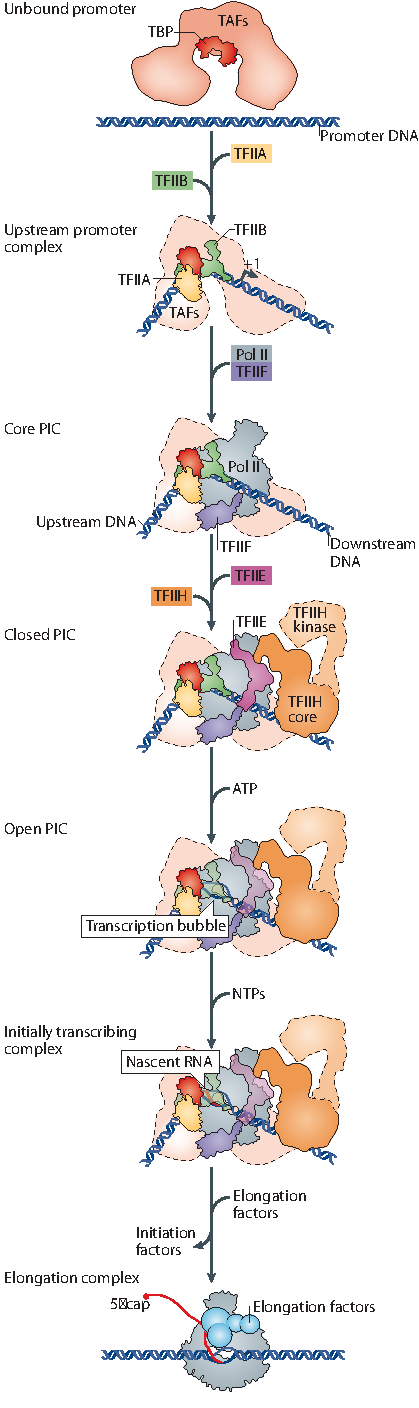
\includegraphics[width=5.095cm]{figures/introduction/picAssembly} % 5.094cm
\caption[Stepwise PIC assembly]{
Stepwise assembly of general transcription factors and \gls{pol2} on a promoter.
adapted from \cite{sainsbury:2015:structural}.
}
\label{fig:picAssembly}
\centering
\end{wrapfigure}
the ternary complex\footnote{The ternary complex is defined as the three-way interaction between DNA, RNA, and \gls{pol2} that forms within transcribing polymerases} required for transcription cannot yet form.
TFIIE and TFIIH are recruited to the \gls{pic} to solve this problem.
TFIIE acts as a bridge between \gls{pol2} and TFIIH, who contains an ATPase module and is able to unwind promoter DNA \citep{holstege:1996:opening}.
This will eventually contribute to DNA melting and the formation of the open \gls{pic}, a structural variant that precedes the shift into elongation.



The order of stepwise assembly of general transcription factors into a functional \gls{pic} was first discovered \invitro{} \cite{buratowski:1989:five}. 
\Invivo{}, however, there is evidence for the activity of the mediator complex in providing additional assembly pathways \cite{esnault:2008:mediatordependent}.
Mediator is a large and flexible protein complex that can interact with virtually every general transcription factor and with \gls{pol2}.
It is known for its fundamental role in transducing regulatory signals from gene-specific transcription factors to the polymerase.
Without Mediator, the \gls{pic} can drive basal transcription levels, but its activity cannot be modulated in response to external factors.
Studies have implicated mediator in the recruitment of TFIIE and TFIIH independently of \gls{pol2}, providing alternative ways to assemble the complete \gls{pic}.
Additionally, interactions between \gls{pol2} and mediator were found to be required for transcription \invivo{} \cite{soutourina:2011:direct}.

After the assembly of the \gls{pic} and the Mediator complex on the promoter, \gls{pol2} relies on TFIIH to relax DNA and physically separate the two strands, creating what is referred to as the transcription bubble.
Studies in human report that once the bubble first opens, it spans about 7 nucleotides.
It then extends forward, allowing the process of transcription to begin.
Polymerases at this stage, however, have to contend with the fact that the RNA-DNA hybrid is too short to be stable.
According to \invitro{} studies, forming a sufficiently long---and therefore stable--hybrid requires several rounds of abortive initiation, where the small RNA is displaced from the template and released.
When the RNA-DNA hybrid reaches a length of about 10 nucleotides, the upstream half of the bubble, which now spans 17-18 nucleotides, collapses, suddenly closing \cite{holstege:1997:three}.
This event marks the detachment of what will eventually become the elongation complex from the scaffold of general transcription factors that is going to be retained at the promoter \cite{pal:2004:role}.

\clearpage
	\section{Elongation} %do these last!
After escaping the \gls{pic}, \gls{pol2} enters the phase of productive elongation.
During this phase, the polymerase travels along DNA, catalysing the addition of nucleotides to the growing RNA molecule that is being synthesised.
The simple addition of nucleotides, however, is not enough to qualify a mature transcript.
Several essential processing steps take place during transcription elongation and contribute to the production of fully formed transcripts.
Among these, the addition of the 5' cap, splicing, and addition of a poly(A) tail all rely on the presence of \gls{pol2} and the \gls{tec} in order to be carried out properly.
The precise composition of the \gls{tec} is poorly understood. 
However, as \gls{pol2} progresses through the transcription unit, several complexes and co-factors are known to dynamically associate with it in order to enact the various maturation steps.  
Transcription elongation is therefore a highly regulated activity that coordinates several different processes to produce mature transcripts.
This regulation is enacted by the cell through several distinct mechanisms, such as the phosphorylation of the \gls{ctd} and the modification of histones.
These very same regulation mechanisms---along with important regulatory sequences---will eventually mark the end of transcription elongation and the transition to transcription termination.

\subsection{Elongation through chromatin}
Chromatin represents an extremely repressive barrier to any kind of DNA based process.
As I briefly touched upon in previous sections, chromatin components---histones---need to be actively dislodged from promoter regions in order to allow the \acrlong{pic} to assemble.
Elongating \gls{pol2} faces very similar problems, as in order to synthesise the RNA, it has to move through an array of nucleosomes without losing contact with DNA.
Although \invitro{} evidence has shown that \gls{pol2} can effectively elongate through a single nucleosome \citep{lorch:1987:nucleosomes}---possibly due to spontaneous disassembly and reassembly of nucleosomes, a process that was recently shown to happen every few seconds\citep{kim:2016:singlemolecule}---the elongation complex alone is not enough to mediate transcription through multiple nucleosomes.

\begin{figure}[ht]

\centering
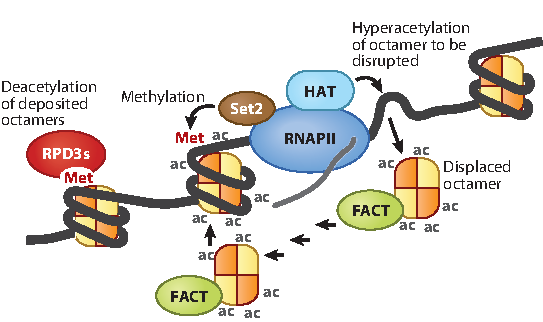
\includegraphics[width=\textwidth]{figures/introduction/nucTranscription}
\caption[Mechanism of transcription through chromatin.]{Overview of the main actors in the mechanism of transcription through chromatin.
Nucleosomes are destabilized through acetylation and chaperoned away---either partially or completely---by \gls{fact} and other complexes.
Addition of methyl groups to histone tails allows the recruitment of \gls{hdacs} and the restoration of chromatin structure.
adapted from \citep{selth:2010:transcript}. }
\label{fig:nucTranscription}

\end{figure}

The \gls{tec} can overcome this problem by enlisting the help of several histone chaperones and chromatin remodeling complexes, as well as by exploiting post translational modifications of histones (Fig: \ref{fig:nucTranscription}). 
The current model for transcription through nucleosomes posits that, depending on the intensity of transcription, histones can either be completely removed from DNA, or be partially destabilized as to allow \gls{pol2} to more easily transcribe through them \citep{kulaeva:2013:mechanism}.
The most notable actors in this phase are \gls{hats} such as Gcn5 and the \gls{fact} (\glsdesc{fact}) complex \citep[for review see:][]{reinberg:2006:de}. 
\gls{hats} are posited to travel with the polymerase, depositing an acetyl group on histone tails.
This has the consequence of destabilizing intra-nucleosome interactions, resulting in a more relaxed chromatin structure and more unstable nucleosomes.
Once histones are acetylated, \gls{fact}---also travelling with the polymerase---destabilizes the H2A-H2B dimer \footnote{
Two of the four core components of a histone. Histones are composed of two H2A-H2B dimers and one H3-H4 tetramer arranged in a symmetrical structure. 
}, removing it and facilitating transcription through the remaining incomplete nucleosome structure. 

Because of the importance of chromatin in preventing spurious initiation, the composition, modifications, and overall structure of nucleosomes must be reset after the passage of \gls{pol2}. 
Specific histone chaperones such as Spt6, together with methil-transferases and \gls{hdacs}, are involved in this process.
First, Spt6 and other histone chaperones reconstruct a complete histone in the wake of transcribing \gls{pol2}.
Subsequently, methil-transferases such as Set2 act by methilating lysine 36 on histone H3. 
Although this modification---unlike acetylation---has no structural consequences on the organization of nucleosomes, it can act as a platform for recruitment of \gls{hdacs}.
The RPD3 complex has high affinity for H3K36 methilation and is recruited immediately after the passage of \gls{pol2} in order to remove the acetyl groups from histones and thus reset the structure of chromatin.

\subsection{Transcriptional pausing}
Nucleosomes do not represent the only obstacle to productive elongation.
A number of occurrences can prevent \gls{pol2} from elongating forward, such as DNA damage, misincorporation of a nucleotide, or collision with another DNA-bound protein.
While the cell has evolved complex---and often slow---mechanisms to deal with the more extreme instances \footnote{For example when DNA is damaged,the cell employs ubiquitinylation and degradation of the largest subunit of \gls{pol2} to resolve pausing.}, transcriptional pausing represents the first and common consequence to all the above-cited events. 
Because reversible pause-inducing events are relatively common during transcription---pausing has been documented in front of every nucleosome \citep{churchman:2011:nascent}---the cell evolved an all-purpose mechanism called backtracking.
The purpose of backtracking is to quickly resolve pausing before the slower, more complex systems are called into action. 

During backtracking---being unable to translocate forward---\gls{pol2} moves backwards, retracing its steps anywhere form 4-5 up to 12-15 nucleotides \citep{cheung:2011:structural}.
This backwards movement causes part of the already synthesized RNA to slide forward into a channel connected to the outside of the complex.
Presence of RNA into the channel promotes the binding of TFIIS \footnote{Also known as \emph{Dst1}} to the complex \citep{cheung:2011:structural}.
This stimulates the intrinsic endonucleolytic activity of \gls{pol2}, which results in cleavage of the extruding RNA and realignment of the 3' end of the nascent transcript with the catalytic site of the polymerase.
At this point, \gls{pol2} has effectively reset its position, having moved back and gotten rid of the extra segment of RNA. 
It can therefore restart its forward translocation and resume the normal catalytic activity.

While this mechanism is a very effective way of dealing with minor pausing events and nucleotide misincorporations, it is not enough to deal with more stubborn pausing agents.
Notably, it has been recently shown that presence of the transcription factor Reb1 on DNA is sufficient to pause the elongation of \gls{pol2} in a way that is unaffected by backtracking; ultimately resulting in the disassembly of the elongation complex and release of the transcript \cite{colin:2014:roadblock}.
 


\subsection{The CTD}
\gls{pol2} and the elongation complex are fundamental elements in coordinating many of the co-transcriptional processes that contribute to the maturation of the nascent RNA.
In order to dynamically recruit all the necessary factors and complexes in a timely fashion, the largest subunit of \gls{pol2} has evolved an unstructured C-terminal domain composed, in \cer, of 26 repeats of the heptapeptide \ctdshort{} \footnote{\ctdlong{} in expanded nomenclature}.
This cluster of repeats can be differentially phosphorylated in different phases of transcription elongation, acting as a dynamically changing interaction surface for different co-factors. 

\subsubsection{CTD phosphorylation dynamics} 
The \gls{ctd} heptapeptide contains a high number of phosphorylatable residues.
Out of the 7 amminoacids, 5 can support the addition of a phosphate group: \tyr{}, \sert{}, \thr{}, \serf{}, and \sers{}.
The combinatorial phosphorylation of \sert{} and \serf{}, however, provides the majority of the functional contribution to transcription elongation and it was recently shown that phospho-groups at these two residues are more abundant than on any of the other residues \citep{suh:2016:direct}. Unlike \sert{} and \serf{}, understanding of the consequences of \tyr{}, \thr{}, and \sers{} phosphorylation is still limited. 
Modification of \thr{} and \sers{} has specialized roles in the transcription of particular species\footnote{In vertebrates, \thr{} has been shown to be important in the processing---but not transcription---of histone genes \cite{hsin:2011:rnap}, while \sers{} was shown to recruit the \gls{ctd} phosphatase Rpap2 specifically to \gls{sns} genes \citep{egloff:2012:role}.}, while the modification of \tyr{} has no attributed roles as of yet. 
In light of this, in the following paragraphs I will focus mainly on the mechanisms and effects of \sert{} and \serf{} phosphorylation.

\begin{figure}[ht]

\centering
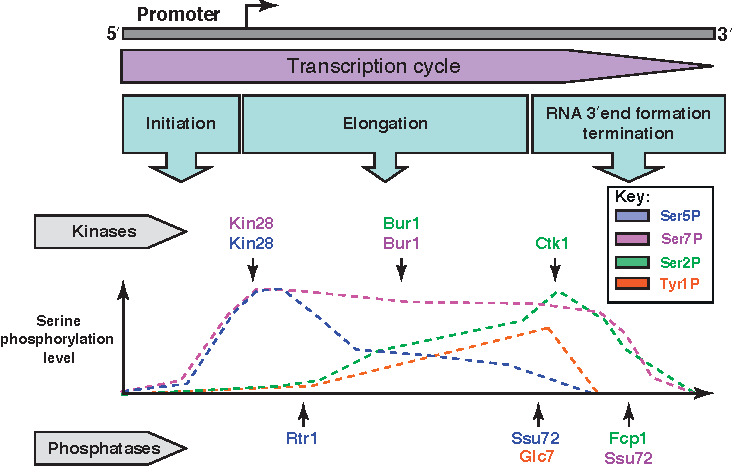
\includegraphics[width=\textwidth]{figures/introduction/ctdPhospho}
\caption[CTD phosphorylation states throughout the transcription cycle.]{
General view of \sert{}, \serf{}, and \sers{} phosphorylation along the transcription cycle,
kinases and phosphatases involved in \gls{ctd} modification are represented immediately above and below the graph.
The two main phosphorylation states, \sert{} and \serf{}, are dominant at the 3' and 5' respectively, reflecting their functional roles in the termination and early elongation phases of transcription.
\sers{} is consistently present throughtout the transcription cycle, but its functional impact in yeast remains elusive. Adapted from \citep{egloff:2012:updating}.
}
\label{fig:ctdPhospho}

\end{figure}

During the Initiation phase of transcription, the \gls{ctd} of \gls{pol2} starts off unphosphorylated (see Fig: \ref{fig:ctdPhospho}).
When the \gls{pic} is fully assembled, Kin28, a catalytic subunit of the general transcription factor TFIIH, phosphorylates the CTD heptapeptide on \serf{}.
In \cer{}, the \gls{ctd} remains mostly \serf{} phosphorylated for the first 450 nucleotides of transcription elongation \citep{mayer:2010:uniform}. 
After this point the combined action of the \serf{}-phosphatase Rtr1 \citep{mosley:2009:rtr1, hunter:2016:phosphatase} and the \sert{}-kinases Bur1 and Ctk1 \citep{qiu:2009:phosphorylation} make \sert{} the most prominent mark \footnote{
It is interesting to note that the phosphorylation state of \gls{pol2} \gls{ctd} is independent of transcript length, but exclusively depends on the amount of nucleotides from the \gls{tss}. 
This will have important implications for the termination of non-coding transcripts.}.
Despite phosphorylation of \sert{} reaching saturation about 600 nucleotides from the \gls{tss} \citep{mayer:2010:uniform}, \serf{} phosphorylation is still present on many repeats, resulting in the presence of a double phosphorylation pattern with important functional consequences (see below).
Only Towards the 3' end of the gene the action of \gls{ctd} phosphatase Ssu72 completely abrogates the \serf{}-P mark, leaving \sert{}-P as the only active mark.
Finally, additional activity of the Fcp1 phosphatase results in the removal of most phospho-marks from the \gls{ctd}, readying the polymerase for another round of transcription.

%Recent studies tried to explore the differences between distal and proximal \gls{ctd} repeats, 
\subsubsection{Functional interactions}

As I outlined above, the transcription cycle follows specific patterns of \gls{ctd} phosphorylation: unphosphorylated \gls{ctd} is recruited to promoter regions, \serf{}-P dominates during early elongation and gradually makes way for \sert{}-P, which is the dominant mark in the later stages of transcription. Each of these stages comes with the potential to interact with numerous co-factors and provides modularity to the elongation complex.

The unphosphorylated state of free-form \gls{pol2} \gls{ctd} allows the polymerase to interact with the mediator complex; an interaction that is thought to contribute to the recruitment of \gls{pol2} to active promoters. 
Once the \gls{pic} is assembled, the polymerase needs to escape the promoter and leave the \acrlong{pic} behind.
The modifications that take place at this stage, namely \serf{} phosphorylation, are thought to disrupt the interaction between \gls{pol2} and mediator---thereby allowing promoter clearance---although evidence remains inconclusive \citep{so:2007:hyperphosphorylation, davis:2002:structure}.

The presence of \serf{} mark during early elongation has two direct consequences: it stimulates capping of the nascent transcript through recruitment of the capping enzymes, and it has the potential to promote early transcription termination through the recruitment of the \gls{nns} complex.
While capping is ubiquitous and required to prevent premature degradation of the transcript, early termination is a quality control mechanism that requires (in addition to \serf{}-P) the presence of specific sequence elements on the nascent transcript and will be described in detail in a future section.

Studies in mammals have reported that the \gls{ctd} is required for splicing to occur properly, in particular heptapeptides containing both \serf{} and \sert{} phopshorylation are known to recruit several splicing factors. Recent studies in \cer{}, however, show differential phosphorylation patterns in intronless and intron-containing genes, hinting at a possible splicing role for \gls{ctd} phopshorylation in yeast \cite{milligan:2016:strandspecific}.

Towards the end of the transcription cycle, \sert{}-P becomes the most prominent mark. 
This phase sees the recruitment of a number of different actors.
Chromatin remodelers and histone modifying complexes such as Set2 and Spt6 are recruited through the \gls{ctd}, making sure that the structure of nucleosomes is maintained.

Finally, 3' end processing, termination, and export are all affected by the \gls{ctd}. binding of components of the cleavage and polyadenylation complex such as Pcf11 and Rtt103 stimulates the termination of transcription and the processing of the transcript 3' end (such as poly(A) tail addition), while recruitment of export factors such as Yra1 direct a rapid and efficient export to the cytoplasm.
 


\clearpage
	 %do writing new stuff in the morning, fixing in the afternoon.
%reset in case acronyms are cited previously, this is their main paragraph and the acronym needs to be in long form.
\glsreset{cpf}
\glsreset{nns}
After its synthesis and maturation are complete, the nascent RNA molecule must be released from the DNA template, and the elongation complex must be disassembled and its components recycled.
In \cer{}, transcription termination is enacted by several widely different mechanisms.
Two predominating pathways terminate the vast majority of transcripts generated by \acrlong{pol2}: the \gls{cpf} pathway and the \gls{nns}  pathway. 
Both these mechanisms rely on short sequences on the nascent RNA---coupled with specific modifications on the \gls{ctd} of \gls{pol2}---to recruit specific factors and enact the disassembly of the elongation complex and the release of the transcript in the nucleus.

In addition to the two main pathways cited above, several non-canonical termination mechanism have been described.
these mechanisms are dedicated to the termination of specific RNA species, or can act as backups when the main pathways fail.


Finally, transcription termination is strictly intertwined with some steps of 3' end processing and maturation, strongly influencing the fate of the transcript. 
%The \gls{cpf} complex couples termination with a polyadenylation step and export competence of the RNA was shown to require this termination mechanism. 
%On the other hand, \gls{nns} is known to lead to either processing (for certain species such as \gls{sns} and \gls{snos}) or complete degradation of the transcript.



\section{The CPF-CF pathway}
The \gls{cpf} pathway was the first termination mechanism described in \cer{} because of its association with the termination of protein-coding genes\footnote{Its activity can extend to certain kinds of non-coding transcripts as well (see \ref{pervasiveTranscripts} for details)}. 
\gls{cpf} termination is unique as it results in cleavage of the nascent RNA before termination occurs.
The site of cleavage is specified through sequence elements present on the nascent RNA and plays an important role in kickstarting the termination reaction.

The main actor of this termination mechanism is the \gls{cpf} complex, a large assembly of modular sub-complexes that act in concert to execute all the required steps. 
This complexity makes \gls{cpf} the most reliable, efficient, and precise termination mechanism in \cer{}.

%There exist some controversy about how \gls{cpf} termination mechanistically occurs.
%The literature proposes two models that explain termination through the \gls{cpf} pathway.
%The allosteric model argues that transcription through the cleavage site leads to conformational changes in the elongation complex, leading to destabilization of the complex and eventually termination.
%On the other hand, the torpedo model posits that after cleavage, the uncapped 5' end of the polymerase-associated transcript is attacked by exonuclease Rat1, leading to the dismantling of the complex through destabilization of the ternary complex once Rat1 catches up with the polymerase.



\subsection{Recruitment and assembly}
\TODO{figure}
Recruitment and initial assembly of the \gls{cpf} complex onto the nascent RNA is promoted by two mechanisms: interaction with specific sequences elements, and interaction with the polymerase \gls{ctd}.

A key component of the \gls{cpf} complex, Pcf11, contains a peptide sequence able to recognize the \gls{ctd}. This \gls{cid} is able to specifically recognize the \sert{}-phosphorylated version of the heptapeptide.
Given the nature of this \gls{ctd} modification---which is confined to the later stages of transcription---density of the \gls{cpf} complex around the polymerase is selectively increased where the complex is more likely to be needed for termination (i.e. at the 3' end of transcription units), facilitating the eventual binding of \gls{cpf} to the sequence elements on the nascent RNA.

Unlike in human, where the cleavage site is defined by a single highly conserved hexanucleotide sequence on the nascent RNA, Yeast \gls{cpf} complex recognizes a number of degenerate short sequences.
Two sub-complexes of \gls{cpf}, \gls{cf1a} and \gls{cf1b}, are responsible for the recognition of these sequences.
In particular, Rna15 and Hrp1 (components of \gls{cf1a} and \gls{cf1b} respectively) directly bind the nascent RNA.
Associated factors Rna14 and Pcf11 contribute to the assembly of the whole complex by interacting with \gls{pol2} and forming a scaffold that serves to tether the catalytic portion of the \gls{cpf} complex to the cleavage site.

The bulk of the catalytic activity of the \gls{cpf} complex is contained in the \gls{cpfa} sub-complex.
\gls{cpfa} directly contacts the cleavage site with its Ysh1 subunit and is responsible of the cleavage of the nascent RNA, one of the events that is thought to kickstart the termination reaction.
\gls{cpfa} also coordinates the polyadenylation reaction through the subunits Yth1 and Fip1. 
These factors recruit and tether the poly(A) polymerase Pap1 to the complex, which will begin catalyzing the addition of a poly(A) tail after the transcript has been cleaved.

Despite the wealth of knowledge available on the mechanics of \gls{cpf} recruitment and assembly, some controversy still surrounds the actual termination mechanism.
Two main models describing the termination reaction exist in the literature, the allosteric model and the torpedo model.

\subsection{The allosteric model}

After cleavage and release of the nascent RNA, the elongation complex has successfully accomplished its job in the transcriptional process and is ready to be disassembled.
The allosteric model is one of the two main mechanistic models that describes the process by which the \gls{tec} is removed from the DNA template.

The allosteric model argues that cleavage is a dispensable signal, and that termination can happen independently of this step.
It posits that after transcription of the cleavage site, \gls{pol2} loses a lot of factors that qualify the elongation complex as such.
The loss of these ``anti-terminator" factors---components of the elongation complex that would prevent termination from occurring---would trigger conformational changes, destabilize the polymerase, and allow components of the \gls{cpf} complex itself to elicit the disassembly of \gls{pol2} from the template.

Several studies support this model. 
\gls{pol2} was shown to lose a number of associated elongation factors after reaching the 3' end \citep{kim:2004:transitions}.
In addition, the component of the \gls{cpf} complex Pcf11 was shown to be able to terminate the polymerase \invitro{} by binding the nascent RNA and the \sert{}-phosphorylated moiety of \gls{pol2} \citep{zhang:2005:ctddependent}.
Ulterior support to this last study was provided by the same authors two years later, when they discovered that Pcf11 is able to perform the same feat in drosophila \citep{zhang:2006:pcf11}.
Finally, a very recent study published on Molecular Cell was able to reconstitute transcription termination in an \invitro{} system in the absence of cleavage \citep{zhang:2015:polya}.

\subsection{The torpedo model}



According to the torpedo model, cleavage represents the main termination signal for the \gls{cpf} complex, as it leaves an uncapped 5'-P on the transcript associated with the still transcribing elongation complex.
These unprotected 5' is the substrate of \FtoT{} exonucleases, a class of enzymes that are known to progressively degrade RNA polypeptides.
The \FtoT{} exonuclease Rat1 was discovered to be associated with the \gls{cpf} complex and is thought to attack the 5' moiety of the \gls{pol2}-associated transcript, starting a processivity race with \gls{pol2}.
Upon winning the race, Rat1 would destabilize the structure of the ternary complex within the polymerase, causing it to break apart and detach from the DNA template.

There are several lines of evidence that support this model for \gls{cpf} transcription termination.
Both Rat1 and its human homolog Xrn2 exhibit termination defects in model cases when mutated \citep{kim:2004:yeast, west:2004:human}.
Furthermore, Rat1 and its co-factor Rtt103 were found to be strongly associated with the 3' end of genes and in physical association with the \gls{cpf} complex \citep{kim:2004:yeast,luo:2006:role}, supporting the idea of a functional recruitment to zones of active transcription termination.
Homology studies found that homologs of Rtt103 in both humans and \cele{} have roles in transcription termination \citep{morales:2014:kub5hera, cui:2008:genes}.
Finally, recent mechanistic studies \invivo{} have demonstrated the kinetic competition between Rat1 and the elongation complex. By employing mutant polymerases that elongate faster or slower than the wild type version, the authors were able to show that slower polymerases result in earlier termination, consistent with the notion that Rat1 needs to physically catch up with the polymerase in order to elicit termination \citep{fong:2015:effects}.

At the same time, several reports argue against the torpedo model as sole effector of transcription termination.
\emph{In vitro} studies were unable to reproduce the termination effect observed \invivo{} using only Rat1  \citep{dengl:2009:torpedo}. More recent ventures re-attempted the \invitro{} approach with limited success  \citep{park:2015:unraveling}, but managed to demostrate that Rat1 is able to terminate polymerases that are destabilized by nucleotide misincorporation.
Several additional mechanistic studies showed that the exonucleolytic activity of Rat1 is unable to mediate the release of the polymerase from the template \citep{luo:2006:role, pearson:2013:dismantling}.
Moreover, termination defects caused by Rat1 mutants were not associated with stabilization of the \gls{pol2}-associated transcript, arguing against the model.
%Finally, recent genome-wide studies were unsuccessful in detecting a widespread effect of Rat1 human homolog (Xrn2) in transcription termination\citep{nojima:2015:mammalian}.


\begin{figure}[ht]

\centering
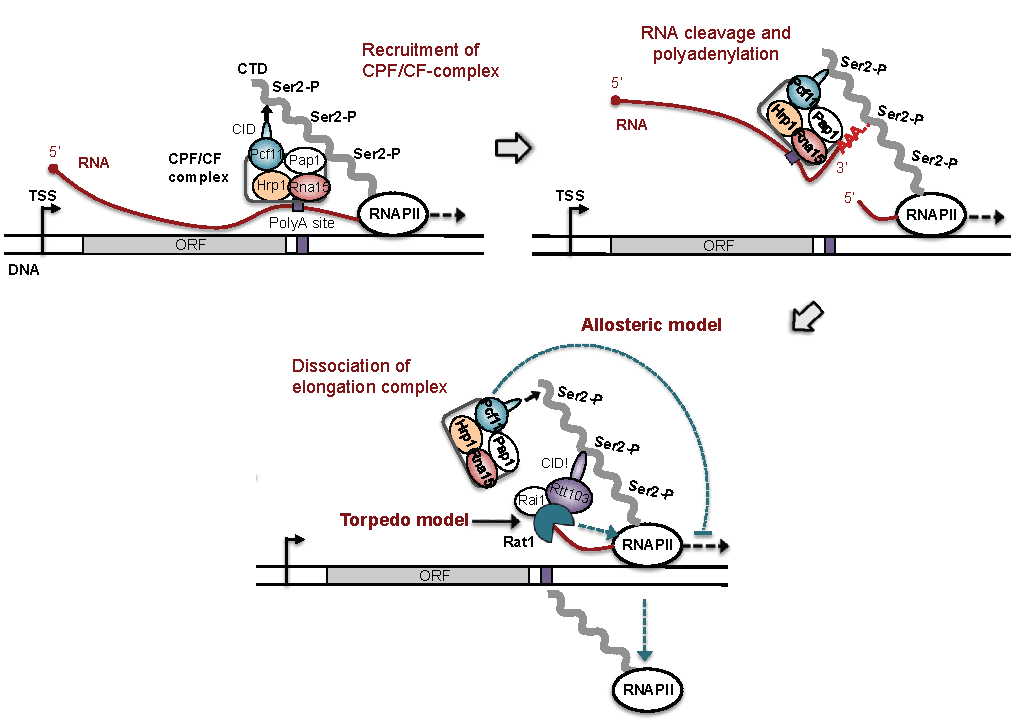
\includegraphics[width=\textwidth]{figures/introduction/cpf}
\caption[Mechanism of CPF-CF termination]{Overview of the main mechanistic step that lead to CPF-CF termination. The complex is recruited thanks to CTD phosphorylation and binding sites on the RNA. The transcript is then cleaved and the elongation complex terminated in accordance with the torpedo or allosteric model.}
\label{fig:cpfTermination}

\end{figure}

\subsection{A unified view of CPF-CF transcription termination}

As evidence for and against the two models piles up, a unified view that combines elements of both torpedo and allosteric model is taking shape.
While the effect of Rat1 on transcription termination (of at least some transcripts) is established, its role as main effector of \gls{cpf} termination has been repeatedly called into question.
Several studies have now described interdependencies between Rat1 and other subunits of the \gls{cpf} complex---notably Pcf11---and the perceived nature of Rat1 is shifting towards that of a molecular effector  that is integrated into a larger system.
The proof of principle that termination is possible without cleavage has been recently provided---albeit \invitro{} \cite{zhang:2015:polya}---and presence of Rat1 has been convincingly shown to facilitate termination \cite{fong:2015:effects}, arguing for a model that integrates these two mechanisms.

%Despite recent advances and the rise of a unified model for transcription termination, mechanistic details on the termination reaction and what prompts it are still sorely lacking.



\section{The NNS pathway}

NNS dependent transcription termination is the second of the main termination mechanisms in S.cerevisiae. 
It is essentially involved in the termination of small Nuclear RNAs (snRNAs), small Nucleolar RNAs (snoRNAs) and a number of other non-functional non-coding RNAs.
It sets itself apart from CPF-CF termination in a number of ways.
First and foremost, it relies on a completely different---and much smaller---set of proteins: the two RNA binding proteins Nrd1 and Nab3 \cite{conrad:2000:yeast}, together with the helicase Sen1. 
Because of the different molecular effectors, the termination mechanism---although still not fully elucidated---is appreciably different. 
Termination is not associated to cleavage of the nascent RNA, and release of the transcript occurs upon disassembly of the elongation complex itself \cite{steinmetz:2001:rnabinding}. 
As a consequence, the 3’ end of the terminated transcript coincides with the termination sites on DNA. 
The NNS complex also distinguishes itself because of the different fate imposed on the RNA released: instead of being exported to the cytoplasm after polyadenylation, the transcripts released are subjected to the activity of degradation enzymes (the nuclear exosome, see below) \cite{vasiljeva:2006:nrd1}. 
To this end the NNS complex recruits both the nuclear exosome and a specific set of 3' end processing factors known as TRAMP (Trf4/Air2/Mtr4p Polyadenylation), which drives polyadenylation and stimulates degradation \cite{lacava:2005:rna, vasiljeva:2006:nrd1}.

NNS termination operates mainly on non-coding RNAs and is generally restricted to the early stages of transcription elongation. 
Despite not being directly involved in the termination of protein-coding genes, it can play a role in the regulation of gene expression by acting as an attenuator \cite{arigo:2006:regulation}(i.e. terminating some transcription events, preventing them from producing functional RNAs), like in the case if IMD2 or URA2 genes \citep{jenks:2008:properties}, or otherwise terminating transcription of non-coding RNAs that might be involved in regulation \cite{thompson:2007:cytoplasmic}.



\subsection{The NNS complex}

The main molecular effectors of the NNS complex are the three protein Nab3, Nrd1, and Sen1.


\paragraph{Nab3}

This factor was originally identified as a polyadenylated RNA binding protein. 
Nab3 contains several structural domains: a conserved RNA Recognition Motif (RRM) that can contact specific sequence elements on the nascent RNA, a region necessary for the interaction with Nrd1, and an essential Glutammine/Proline region at the C-terminus.

Biochemical experiments have shown that Nab3 forms a stable heterodimer with Nrd1 and contacts the RNA as such \cite{conrad:2000:yeast}. 
In addition, the structure of the RRM has been solved, revealing the structural basis for the preference of the sequence UCUUG \cite{lunde:2011:structural}. 
Finally, its Glutammine/Proline region---despite being generally unstructured---can assemble into amyloid structures \cite{orourke:2015:amyloidlike}.


\paragraph{Nrd1}

Identified as part of the ``nuclear pre-mRNA downregulation" family of proteins, Nrd1 is the most abundant of the three members of the complex. 
Its main features consist of an RRM structure that allows it to contact the nascent RNA, a CTD interaction domain (CID) that mediates the interaction with RNAPII (see below) and a Nab3 interaction motif that allows it to form a stable heterodimer.

Nrd1's RRM was shown in vivo to contact the consensus sequence GTA[A/G] \cite{steinmetz:1998:control}. 
Recent in vitro studies, however, have shown that several other G-rich and A-rich sequences could be bound equally well \citep{bacikova:2014:structure}, although the in vivo relevance of these studies remains to be demonstrated. 

In addition to the RNA, Nrd1 can contact RNAPII through its CID \cite{kubicek:2012:serine,vasiljeva:2008:nrd1nab3sen1}. 
Although dispensable for cell viability, the CTD-CID interaction is required for efficient termination (see below).

Curiously, Nrd1 also contains a Glutammine/Proline region at the C-terminus, similarly to Nab3. 
Deletion of this region shows no growth or termination defects, but is synthetic lethal if combined with other aphenotypic mutations on Nab3 [our unpublished data]. 
The functional implications of these genetic interactions are still unknown.
 

\paragraph{Sen1}

This extremely large (253kDa) and very low abundance (125 molecules per cell) protein is the only member of the NNS complex to have enzymatic activity \cite{steinmetz:1996:repression}. 
Sen1 was characterized as a helicase of the SFI superfamily and is very closely related to Upf1, a member of the Non-sense Mediated mRNA Decay (NMD) pathway in the cytoplasm. 
Unlike its close relative, Sen1 possesses a nuclear localization signal and acts in the nucleus, where it can physically interact with the other members of the NNS complex Nrd1 and Nab3. 

Structurally, Sen1 contains a helicase domain able to hydrolize ATP and a large N terminal domain. 
The helicase domain was recently purified in E.coli and biochemically analyzed, revealing binding affinity for both DNA and RNA, but a slower translocation rate on RNA \cite{martintumasz:2015:saccharomyces}. 
Moreover, its ATPase activity was shown to be necessary for termination in vitro \cite{porrua:2013:bacteriallike}. 
The N-terminal region of Sen1 was implicated in the interaction with the RNAPII, as well as other factors such as Rnt1 and Rad2, but the implications of the latter interactions remain obscure.

\subsection{The mechanism of transcription termination}

As in the case of CPF-CF, the NNS complex is recruited to the region of termination through two distinct mechanisms that cooperate to maximize efficiency: the CTD of the polymerase \cite{vasiljeva:2008:nrd1nab3sen1} and specific sequence elements on the nascent RNA \cite{conrad:2000:yeast}. 
Within the NNS complex, Nrd1 and Nab3 are the major interactors of these elements, providing specificity and ensuring that Sen1---believed to be the molecular effector of NNS termination---is recruited only in the appropriate circumstances \cite{porrua:2013:bacteriallike}.

The CTD of RNAPII is contacted by the CID domain of Nrd1. 
This domain preferentially recognizes the Ser5-phosphorylated variant, which is the prevalent CTD phosphorylation state in the first 500-600 nucleotides of transcription. 
This preference confers to the NNS complex a high degree of specificity for terminating transcription in the early stages of elongation. 
According to the current model for NNS termination, the interaction with the CTD occurs prior to RNA binding, and facilitates recognition of sequence elements on the nascent transcript.  
Presence of Ser5-P CTD was shown to be a pre-requisite for efficient termination, as placing high efficiency NNS binding sites at the end of long transcription units---where the levels of Ser5-P would be completely supplanted by Ser2-P---does not result in termination \cite{gudipati:2008:phosphorylation}.

\begin{figure}[ht]

\centering
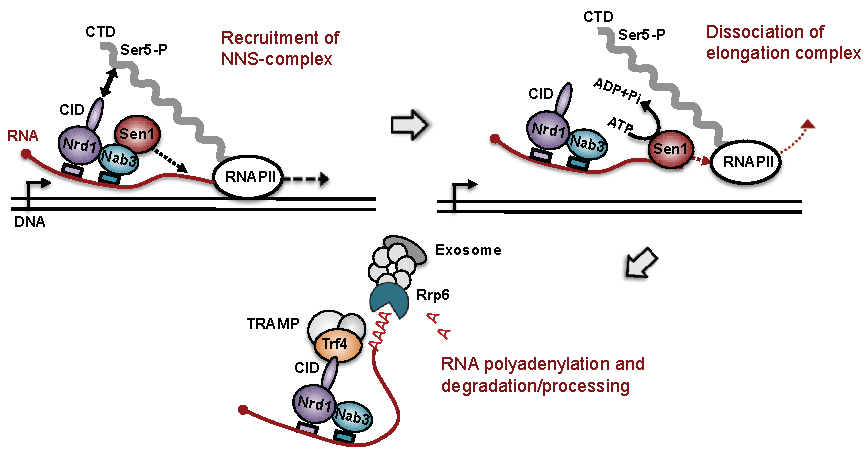
\includegraphics[width=\textwidth]{figures/introduction/nns}
\caption[Mechanism of NNS termination]{Main stages of NNS-dependent termination. the NNS complex is recruited thanks to \serf{}-phosphorylated CTD and sequence elements on the transcript. Termination is elicited by Sen1, presumably by translocating along the transcript. Finally, the exosome is recruited to the transcript and the transcript is either trimmed or completely degraded.}
\label{fig:nnsTermination}

\end{figure}

Recruitment of Nrd1 to the CTD, however necessary, is not sufficient to trigger termination. 
The Nrd1-Nab3 heterodimer must also contact the nascent RNA through the RRM domains of the two subunits.
Original studies have investigated the sequence elements that drive NNS termination, pinpointing two core consensuses: UCUU as the main binding site for Nab3, and GUA[A/G] as the main site for Nrd1 \cite{carroll:2004:identification}. 
More recent investigations redefined these consensuses and identified new sequence elements that can increase termination efficiency when in proximity of canonical binding sites. 
Use of an in vivo SELEX (Systematic Evolution of Ligands by Exponential enrichment) strategy allowed to extend the core consensus sequences for both Nrd1 and Nab3 with nucleotides that proved critical for binding (see fig ??) \cite{porrua:2012:in}. 
In addition, AU-rich sequences found downstream of Nrd1 sites were shown to play a role in increasing both termination efficiency and recruitment of Nrd1 \cite{porrua:2012:in}. Similar conclusions have been reached by in vivo crosslinking studies \cite{wlotzka:2011:nuclear}.

Despite the efforts expended in identifying sequence elements that could univocally lead to NNS termination, a lot of ambiguity remains on what constitutes an NNS terminator \invivo{}. 
While presence of Nrd1-Nab3 binding sites is required, no consistent pattern emerges in number, spacing, or quality of Nrd1/Nab3 sites at known NNS termination sites. 
Despite this, In vitro studies on model cases have identified some features of heterodimer binding. 
For example, mutation of Nab3 binding sites proved to be more deleterious to heterodimer recruitment than mutation of Nrd1 sites \cite{carroll:2007:interaction}. 
Moreover, multiple heterodimers were found to bind the same RNA sequence, possibly cooperatively  \cite{carroll:2007:interaction}. 
It remains impossible, however, to generalize these results beyond the few sequences tested. 
While the NNS complex could simply rely on a high number of low affinity sites to reach an occupancy threshold, it remains possible that several unseen elements play a role in qualifying NNS terminators, influencing the quantity and quality of Nrd1 and Nab3 binding sites necessary for an efficient termination.

When the Nrd1-Nab3 heterodimer is bound to the nascent RNA, the molecular effector of NNS termination, the helicase Sen1, is recruited to the complex. 
Studies have shown that Sen1 is strictly required to terminate transcription, but the mechanism through which this happens is not clear. 
Significant advances in the understanding of this phenomenon came from use of an in vitro transcription termination system \cite{porrua:2013:bacteriallike}. 
In this context, Sen1 alone was found to be sufficient to disassemble the elongation complex. Termination was shown to occur preferentially at sites of pausing and to require both the interaction of Sen1 with the nascent transcript and ATPase activity. 
It is unclear whether ATP-dependent translocation of Sen1 on the nascent RNA is required for termination. However, results from an in vivo study suggest the existence of a kinetic competition between transcription elongation and Sen1 translocation on the RNA. 
The authors investigated the effect of the speed of transcription on NNS termination, showing that faster transcription results in longer NNS-terminated transcripts, while slower transcription produces shorter transcripts and is able to suppress mutations on Sen1 \cite{hazelbaker:2013:kinetic}. 
Taken together, these results support a model where, akin to the bacterial termination factor Rho, Sen1 would contact the nascent transcript and translocate in a 5’ to 3’ direction, eliciting termination upon catching up with the polymerase.

\subsection{Processing of products of the NNS pathway}

The process of NNS termination is strictly connected with 3' end processing or degradation mediated by the nuclear exosome, a multiprotein complex endowed with exonuclease activity \cite{vasiljeva:2006:nrd1}. 
The exosome plays a major role in nuclear RNA quality control, degrading aberrant transcripts, a number of non-functional non-coding RNAs, and trimming the precursors of functional small non-coding RNAs such as sn/snoRNA \cite[for review see][]{kilchert:2016:regulation}. 
The exosome is composed of six non-catalytic subunits arranged in a ring-like structure, together with three cap subunits that can bind RNA (see figure X). 
The catalytic activity of this complex is dependent on two active 3' to 5' exonuclease, Dis3 and Rrp6. 
Dis3 associates with the ring on the opposite side of the three cap subunits, and degrades RNAs that are threaded through the cap proteins and into the ring \cite{makino:2015:rna}. 
The exosome is present throughout the nucleus and in the cytoplasm. 
However, only the nuclear version can associate with the other exonuclease, Rrp6, whose activity is known to regulate the levels of many NNS targets.

Recruitment of the exosome to NNS targets takes place via one of the exosome’s co-factors: the TRAMP complex. 
TRAMP (for Trf4/Air2/Mtr4p Polyadenylation) is a nuclear complex composed of the poly(A) polymerase Trf4, the RNA-binding protein Air2 and the helicase Mtr4. 
Trf4 is the core subunit of the complex, to which both Air2 and Mtr4 bind independently. 
It possesses poly(A) polymerase activity, but unlike Pap1---the canonical poly(A) polymerase associated with the CPF-CF complex---it can only add tails in a distributive manner. 
Trf4 is also the factor responsible for the coordination between the NNS complex and the nuclear exosome. 
A recent study showed that Trf4 contacts Nrd1 through a small motif called Nrd1 Interaction Motif (NIM) . 
The NIM on Trf4 mimicks Ser5-P CTD and can therefore compete with the CTD of RNAPII for the interaction with the CID (CTD interaction domain) on Nrd1. 
The interaction of Nrd1’s CID with the CTD and Trf4 are mutually exclusive, and Trf4 was shown to have much higher affinity for the CID. 
These findings have suggested a model whereby TRAMP is recruited to the RNA when the CID of Nrd1 is freed from the CTD of the polymerase \cite{tudek:2014:molecular}. 
This effectively allows the coordination of events going from termination to the handover of the transcript to TRAMP and the exosome.

As a co-factor of the exosome, TRAMP is able to both recruit and stimulate its activity. 
Addition of a poly(A) tail to the terminated transcript is thought to provide an unstructured platform that can be easily be threaded through the non-catalytic subunits of the exosome. 
However, TRAMP has been known to stimulate exosome activity even indipendently of poly(A) polymerase activity \cite{tudek:2014:molecular}. 

By virtue of the tight connection between NNS and TRAMP, NNS-terminated transcripts are usually subject to rapid degradation. SnoRNAs and snRNAs constitute notable exceptions, in that they are heavily structured functional non-coding transcripts that are recruited to the exosome, but undergo only trimming of their 3’ ends instead of complete degradation. This is thought to occur thanks to the presence of secondary structure and additional proteins binding the RNA, preventing the transcript from being entirely threaded through the exosome \cite{mitchell:1997:exosome}.


\section{Non-canonical termination pathways}

CPF-CF- and NNS-dependent termination seemingly account for the vast majority of RNAPII transcription termination events in the cell.
Several additional mechanisms, however, can terminate transcription in S.cerevisiae. 
These non-canonical termination pathways are generally thought to act as a fail-safe pathway in restricting readthrough transcription \cite{colin:2014:roadblock,ghazal:2005:genomewide}.


\subsection{Rnt1-dependent termination}

The yeast Rnase III homologue Rnt1 is an enzyme that binds and cleaves double-stranded RNA stem-loops at a defined recognition site. 
Rnt1’s known function in the cell is that of cleaving polycistronic rRNAs and snoRNAs transcripts, promoting their subsequent trimming and processing by the exosome \cite{ghazal:2005:genomewide}. 
Recently, Rnt1 binding sites have been identified downstream of a number of genes and its cleavage activity has been implicated in transcription termination.

Studies on the model gene NPL3 have shown that deletion of Rnt1 leads to transcriptional readthrough and can even mediate the production of dicistronic transcripts \cite{ghazal:2009:yeast}. 
Rat1, the mediator of the CPF-CF termination according to the torpedo model, was found to be also required for proper termination by Rnt1. 
This led to a model where Rnt1 cleaves a stem-loop that forms downstream of the CPF-CF cleavage site, generating a non-polyadenylated transcript, and leaving an uncapped 5’ on the nascent transcript. 
This free 5’-OH is a substrate for exonuclease Rat1, and transcription termination is thought to occur with a mechanism akin to the CPF-CF torpedo model, with Rnt1 as the cleaving agent instead of the CPF complex  \cite{ghazal:2009:yeast, rondo:2009:failsafe}.

The termination mechanism is usually very intimately connected with 3’ end processing and with the fate of the transcripts it produces. The case of Rnt1-dependent termination, however, is peculiar in this respect.
Use of in vivo reporter systems showed that, in the absence of a polyadenylation site, Rnt1-dependent transcripts are unstable and supposedly targeted by TRAMP and the exosome \cite{ghazal:2009:yeast}. 
However, addition of a cryptic polyadenylation site close to the Rnt1 binding site in the same system results in increased transcript stability that is Pap1-dependent. 
This suggests that depending on its environment, Rnt1 can either stimulate the usage of a nearby Polyadenylation site or produce transcripts that are targeted for degradation \cite{rondo:2009:failsafe}.

\subsection{Road-block termination}
  
Road-block termination represents another non-canonical mechanism that can mediate transcription termination. 
Road-block was first observed as a termination mechanism for RNAPI, where  a DNA binding factor acts as a physical obstacle for the polymerase. 
The polymerase is thought to stall at the DNA binding site and eventually dissociate from the template through unclear mechanisms \cite{lang:1994:model, lang:1993:reb1}. 

When the mechanism was first described, in vitro work had shown that transcription factor Reb1 was able to pause all three yeast RNA polymerases \cite{lang:1994:model}. 
Later studies from the same authors confirmed that the DNA binding site for Reb1 was coincident with sites of RNAPI transcription termination in vivo \cite{reeder:1999:saccharomyces}. 
Combination of these experiences led to a model where Reb1 is binding DNA and terminating RNA polymerase I at specific rDNA loci. 
It was only in 2012 that a Reb1 paralogue---Nsi1, who binds the same consensus sequence as Reb1---was implicated as the true in vivo effector of RNAPI termination, while Reb1 was proven to not have a role \cite{reiter:2012:reb1homologue}. 

I have participated to a study of the laboratory showing that Reb1 is the effector of roadblock transcription termination for RNA polymerase II in vivo. 
This study will be described in the results section.

\clearpage
	\section{The transcriptional landscape of \cer{}}

%trFactors
\begin{savequote}[70mm]
Uomini, poich\'{e} all'ultimo minuto non vi assalga il rimorso ormai tardivo di non aver piet\'{a} giammai avuta e non diventi rantolo il respiro, sappiate che la morte vi sorveglia\ldots
\qauthor{Fabrizio Simonetti} 
\end{savequote}

\chapter{Transcription factors}


	General Regulatory Factors (GRF) are a subset of abundant, multi-functional DNA-binding proteins involved in several aspects of chromosomal function. In addition to their role as transcriptional activators, GRF are involved in transcriptional silencing, telomere maintenance, and centromere function.

The proteins defined as GRF are Rap1, Reb1, Abf1 and Cbf1. GRF are a functionally and structurally heterogeneous group of proteins, However, they all share Myb-like DNA binding domains. Additionally, GRF have the capability of activating transcription through specific binding in promoter regions and modification of the chromatin structure. Through this mechanism, GRF are known to regulate a substantial number of genes in S.cerevisiae (approx. 10\% for every factor).

In this section, I will describe in brief the specific roles of each GRF and subsequently focus on their transcriptional activity.



\section{Rap1}
The essential transcription factor Rap1 is probably the best characterized GRF and It has a multitude of functions. Rap1 has a strong preference for specific DNA element ACACCCRYACA. This binding is mediated by two large DNA binding domains very similar to those of the human oncogene Myb. 
Rap1 is the main transcriptional activator of ribosomal protein (RP) genes, controlling the expression of about 90\% of these species. This regulation is enacted through multiple pathways. First, Rap1 recruits a number of ancillary transcription factors: Fhl1, Ifh1, Sfp1, and Hmo1. Together they modify the structure of chromatin and stimulate transcription (reja and pugh, 2015, molecular). Second, Rap1 is able to recruit TFIIA and TFIID to the promoter of RP genes, accelerating the rate of PIC formation at these loci (Papai, 2010, tfiia).

In addition to its activator capabilities, Rap1 also works as an active silencer of transcription. During vegetative growth, the mating type loci of S.cerevisie are transcriptionally inactive. Their silencing is mediated by binding of Rap1, Orc1, and another GRF, Abf1. These proteins are able to recruit Sir1, Sir2, Sir3, and Sir4, which mediate the spread of heterocromatin over the HML and HMR loci, preventing transcription initiation. The transcriptional repressor activity of Rap1 has also been reported for RP genes under conditions of nutrient starvation, but in these conditions the silencing mechanism remains unclear (reja pugh). 

Lastly Rap1 has been implicated in the maintenance of telomeres. In this context, Rap1 is part of a complex named Telosome together with Rif1 and Rif2. The telosome forms a protective cap around telomere sequences and is required for different aspects of telomere homeostasis such as telomere length regulation, inhibition of telomere end resection, protection from telomere fusion and inhibition of untimely activation of the DNA damage checkpoint (for review see wellinger, 2012). Recent genome-wide studies identified Rap1 binding sites both at telomeres and RP genes, showing that these two classes of binding sites are distinct (rhee and pugh). Somewhat consistent with this notion, another study showed how Rap1 possesses two binding modes. According to the authors, Rap1 can either bind a single site with high efficiency making use of both its Myb-like DNA binding domains, or it can bind more degenerate sequences with lower affinity using only one domain, but forming higher stoichiometry complexes (feldmann and galletto, 2014).
Rap1, together with other GRF such as Reb1 and Abf1, has been shown to have a role as as insulator (i.e. preventing the spread of heterochromatic silencing), and is thought to act in this capacity around both telomeres and mating type loci (fourel and Gilson, 2002, general).

\section{Abf1}

Both Structurally and functionally close to Rap1, Abf1 is another essential factor implicated in numerous processes. Abf1 binds the split DNA site TCN{7}ACG, which is known to regulate hundreds of promoters. 
While the vast majority of RP genes are regulated by Rap1, a cohort representing 10\% of the total is under the control of Abf1. A recent study investigated the mechanism of Abf1-dependent RP gene regulation, showing that Abf1 is found in association with Fhl1 and Ifh1, but has a lower occupancy on the promoter relative to Rap1 (fermi:2016:promoter). Abf1-dependent regulation of RP genes seems to possess distinct features from the canonical Rap1 regulation. Under nutrient starvation, Abf1 was observed to be more stably associated with the promoter and this resulted in a severe downregulation of gene expression. The authors speculated that stable association of Abf1 with DNA could mediate transcriptional silencing, while a more dynamic interaction could mediate activation.

Akin to Rap1, Abf1 is known to act in silencing at the mating type loci, as well as an insulator in sub-telomeric regions (mak et al 2009). 

Abf1 is present in a number of autonomous replicating sequences (hence the name ARS Binding Factor 1). These regions of the genome are essential to the process of DNA replication and act as its starting points. The C-terminal region of Abf1 was found to enhance replicative activity independently of the transcription activation domain (Wiltshire:1997:abf1p). In addition, replication factors have been shown to increase Abf1 DNA-binding activity (feng:1998:saccharomyces). Despite these data, however, Abf1’s mechanism of action at replication origins has never been fully elucidated.

Lastly, Abf1 is implicated in the activity of the global genome nucleotide excision repair mechanism (GG-NER). Abf1 was shown to form a stable complex with Rad7 and Rad16, two essential protein for GG-NER activity (reed:1999:yeast). Additionally, imparing Abf1 DNA binding results in UV-sensitive yeast. The Rad7-Rad16-Abf1 complex is known to generate superhelical torsion in DNA (yu:2004:yeast) , and Abf1 is thought to provide specificity to the complex through its DNA binding activity (Yu:2008:abf1binding).

\section{Reb1}

Reb1 was first identified as an rDNA enhancer binding protein, where it acts in stimulating transcription of ribosomal DNA. Reb1 tightly binds the sequence TTACCCGG with a bipartite myb-like DNA binding domain. Functionally, it acts to promote transcription of about 600 genes and it was implicated as an insulator in sub-telomeric regions. The homologue of Reb1 in S.pombe has been extensively studied as a DNA replication termination factor, as it is able to stall replication forks. The implication in this process in S.cerevisiae, however, is still unproven.

Reb1 was mistakenly believed to be the effector of RNAPI transcription termination (lang reeder). This notion, however, was dispelled when it was shown that Nsi1, a related protein that binds the same consensus on DNA, was the true molecular effector of RNAPI termination (ref, 2012). Interestingly, Reb1 is now implicated in the termination of RNAPII through the same road-block mechanism with which it was thought to terminate RNAPI (colin).

\section{Cbf1}

Cbf1 is the only GRF thus far to not possess a myb-like DNA binding domain. Instead, it is a member of the helix-loop-helix family of DNA binding factors. Cbf1 is mostly known for its activity as a structural element in centromeres, but can stimulate transcription of a limited number of genes.

In S.cerevisiae, centromeres are short (~120 nucleotides) DNA sequences coated with proteins that mediate assembly of the kinetochore and proper chromosome segregation during mitosis. Structurally, the centromere sequence is divided into three Centromere DNA Elements (CDE): CDEI, CDEII, and CDEIII. Cbf1 is the main binder of CDEI, a region of the centromere known to be important, but not essential for chromosome segregation. 


\begin{tabular}[c]{cccp{5.5cm}}
\hline 
GRF & DNA-binding & \makecell{Chromatin\\Remodelling}  & Functions \\ 
\hline 
Rap1 & bipartite Myb-like & RSC & RP genes activation, silencing of mating type loci, telomere maintenance \vspace{3.5mm} \\ 
Abf1 & Myb-like & RSC & RP genes activation, silencing of mating type loci, insulator, stimulator of DNA replication \vspace{3.5mm} \\
Reb1 & bipartite Myb-like & RSC & terminator of RNAPII, insulator \vspace{3.5mm} \\ 
Cbf1 & Helix-turn-helix & unknown & part of centromeres, transcriptional activator \\ 
\hline 
\end{tabular} 

\section{Chromatin remodeling} 
A common feature of GRFs is the capability of altering the local chromatin structure in the vicinity of their binding sites. This mechanism is used to clear nucleosomes from promoters and thus stimulate transcription. As a general rule, GRFs are “obbligate synergizers”: they can weakly stimulate transcription on their own, but achieve a much greater effect when another weak activator binds the same promoter. The chromatin remodeling activity of GRFs is thought to act as a force multiplier, allowing normally weakly binding transcriptional activators to be stably bound on DNA.

Although all GRF described possess some level of chromatin remodeling activity, it is unclear whether it stems from use of a common system. Studies implicated Reb1 and Abf1 in connection with the RSC complex (madhani,2009). To prove this point, the authors inserted a Reb1 site within an ORF observing that an NFR could form and that it required both the presence of Reb1 and that of Sth1, the main subunit of the RSC complex. These findings were mostly confirmed by more recent investigations (kubik,2015), which found a large overlap between promoters regulated by Reb1 and Abf1 and promoters regulated by RSC. The same study, however, discovered a number of promoters where NFRs are generated in a Reb1- and Abf1-dependent manner, but independent of RSC, arguing for a more complex regulation mechanism. In the case of Rap1 and Cbf1, although their effect on chromatin is well known, there are no mechanistic details on how these proteins displace nucleosomes. 

\subsection{GRF and their genome-wide effect on chromatin structure}

The stereotypical view of eukaryotic promoters is characterized by well-positioned +1 and -1 nucleosomes surrounding a 150+ stretch of unbound DNA. This notion was challenged by a recent study that showed the existence of nucleosomal particles inside a large number of promoter NFRs. These fragile nucleosomes (FN) are particularly sensitive to the amount of Micrococcal nuclease (MNase) used to reveal nucleosome positioning in a genome-wide manner, and therefore went undetected until now (kubik). Analysis of the distribution of GRF binding sites relative to promoters showed that fragile nucleosomes are significantly associated with GRF binding. Additionally, the GRF-associated chromatin remodeling complex RSC was implicated in the process, and insertion of GRF binding sites in previously unaffected promoters was shown to induce fragile nucleosome formation. For Reb1 and Abf1, the GRF binding site seems to coincide with the position of the fragile nucleosome, suggesting a kinetic competition between histones and GRFs. In the case of Rap1, however, the situation is less clear. The binding site was detected upstream of the fragile nucleosome, and often entailed the presence of two, not one, of these unstable particles. How such large NFR is generated and how fragile nucleosomes are maintained within it is still unknown. 

Another study recently investigated the effect of GRFs Rap1 and Abf1 on genome-wide chromatin assembly. While chromatin activity has been (expectedly) detected at directly regulated promoters, the two GRFs were shown to affect—albeit to a lesser extent—the chromatin structure of thousands of genes. Using thermosensitive mutants of Rap1 and Abf1 the authors analyzed genome-wide nucleosome occupancy. Analysis of these datasets led to the conclusion that a modest but significant change in nucleosome disposition was happening at a number of loci that were not described as regulated by either Rap1 or Abf1. Upon further analysis, these promoters were found to be enriched in low affinity or degenerate Rap1 and Abf1 sites. This suggests that even low affinity binding of GRFs can contribute to the regulation of gene expression through a chromatin remodeling activity, and underscores the idea of GRFs as obbligate synergizer—or enabler of transcription—on a much larger scale than previously thought. 

\section{GRFs and transcription termination}

Recently, an additional role was described for a number of GRFs in transcription termination of RNAPII. Reb1 was the first GRF to be described in this capacity (colin). It was shown that Reb1 is able to terminate RNAPII through a road-block mechanism that resulted in the disassembly of the elongation complex via degradation by the Rsp5/Cul3 ubiquitin ligases. Another study implicated Reb1, Abf1, and Rap1 in NNS termination as ancillary factors that would stall the polymerase and promote disassembly of the elongation complex by Sen1 (roy:2016:common).

The authors found that several binding sites for GRFs were present downstream of a selected number of SnoRNAs. These binding sites were associated with increases in polymerase occupancy, and the 3’ end of the upstream SnoRNAs were found to cluster in the vicinity of the site (an uncommon occurrence, as SnoRNAs are generally terminated by the NNS pathway, which results in heretogeneous 3’ ends). This led to a model that posits cooperation between NNS termination and GRFs, where the latter would act as a pausing element and allow Sen1 to more easily reach the elongation complex.

 


	\input{chapters/introduction/trFactors/rap1}
	\input{chapters/introduction/trFactors/abf1}


%\part{Results}
%\chapter{Roadblock}
bla bla roadblock

\section{Reb1}
maybe paper here? 

\section{Rap1}

\begin{itemize}
\item detection of rb, how many sites, where, biases
\item detection of specific sites with RB
\item effects of Nrd1-AA and rna15, eventually analysis of surrounding features
\end{itemize}

\section{Other factors rb}

\begin{itemize}
\item systematic analysis of mcisaac binding sites
\item taking into account annotated transcription
\item case of ABf1

\end{itemize}

\section{RB in the genome}

\begin{itemize}
\item tRNAs, already described, but show genome wide data and numbers
\item tRNAs reverse. this is new, show combined peaks and provide numbers
\item centromeres. intro + plots at centromeres on both sides
\end{itemize}



%\chapter{Origins	}
bla bla origins

\section{profiling transcription around origins of replication}

\begin{itemize}
\item asymmetric profile
\item peak in front of ORC
\item antisense perplexing peak
\end{itemize}

\section{termination?}

\begin{itemize}
\item global termination profiling, show controls for reb and rap showing that pA is detectable even in WT
\item effect of NNS
\item effect of CPF
\item Roadblock of ORC, julien's plots

\end{itemize}



\section{effects of endogenous transcription}

\begin{itemize}
\item data description from other paper (efficiencies)
\item effects on firing efficiency
\item effects on timing
\end{itemize}

\section{effects when termination is defective}

see other julien's data? 

\section{ORC does not prevent MCM sliding}

figure containing chip sliding? maybe better to determine peaks on both datasets and then kernel smooth the results.
%\chapter{SELEX}

hopefully paper

\section{•}
%\part{Discussion}

%\part{Materials and Methods}
%\appendix
%\chapter{appendix A}


\singlespacing
\bibliographystyle{acm}
\bibliography{references}
\end{document}